\begin{center}
\Large{T.P.N°3:Acción del Viento CIRSOC 102/205}
\end{center}

\begin{enumerate}
\item Hallar las acciones del viento de la estructura del TPN°2 para el sistema principal resistente a las fuerzas del viento (SPRVF) y además de los componentes y revestimientos (C\&R) según CIRSOC 102/05.\\

\end{enumerate}

\begin{center}
\underline{\large{Solución Ejercicio 1}}
\end{center}

\begin{enumerate}
\item \underline{Descripción y datos del problema}
\begin{itemize}
\item Tipo de estructura: Hangar de aviones.
\item Ubicación: Comodoro Rivadavia - Zona Costera.
\item Tipo de entorno: Abierto.
\item Dimensiones de la planta: 30m x 50m.
\item Altura del alero: 7m.
\item Altura de cumbrera: 11.87m.
\item Altura media: (Altura del alero + Altura de cumbrera)/2 = 9.43m
\item Pendiente $\theta:$ 18°
\end{itemize}

\begin{figure}[H]
\begin{center}
     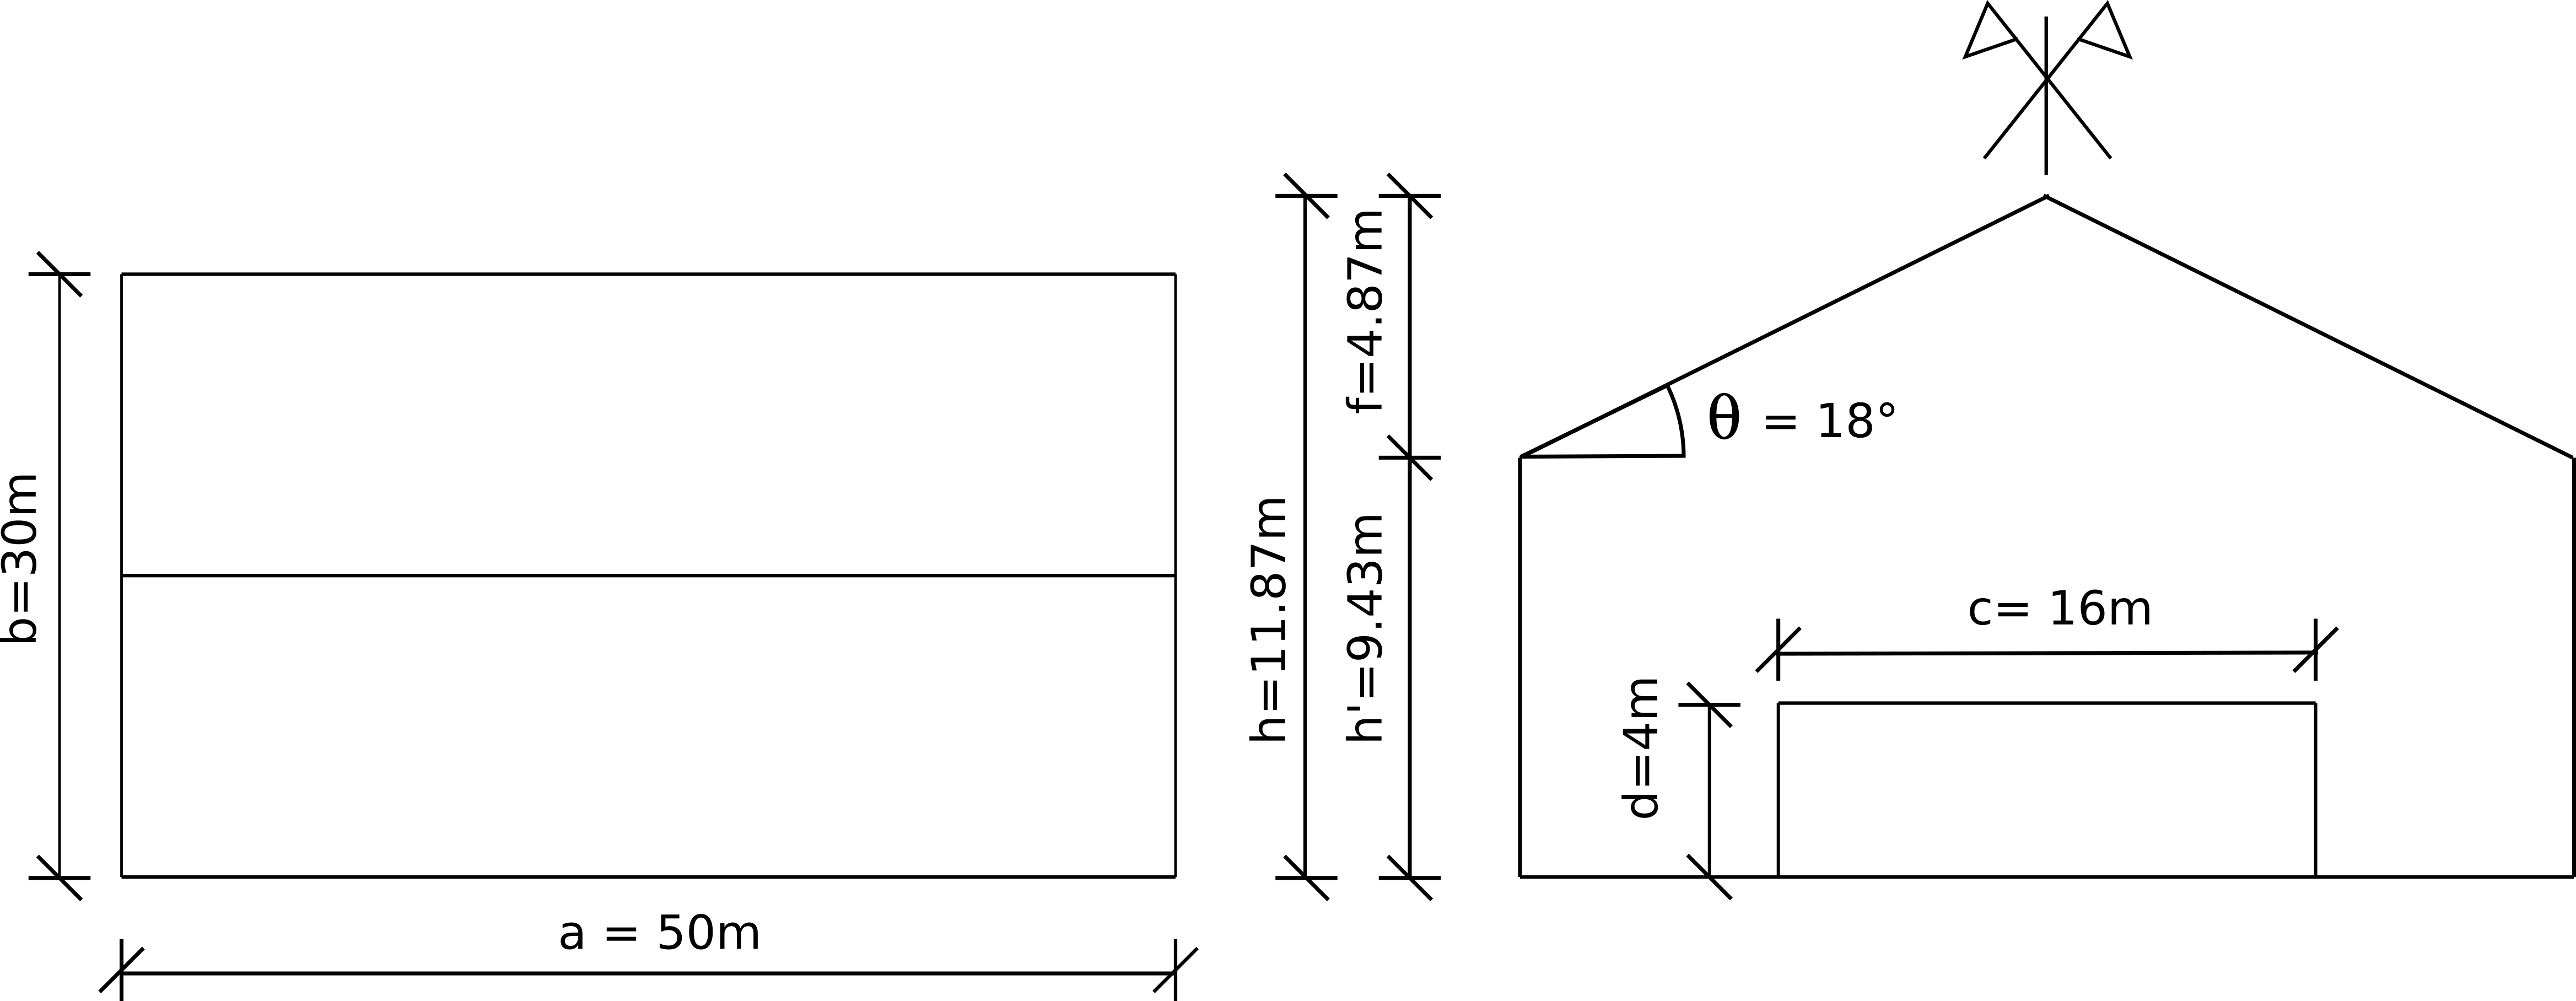
\includegraphics[scale = 0.7]{chapters/chapter_1/images/figura1.png}
\end{center}
\end{figure}

\item \underline{Exposición y clasificación del edificio}\\
El edificio se localiza en la localidad de Comodoro Rivadavia, a 100 metros de la zona costera, correspondiéndole la categoría de exposición D.\\
Su función es el almacenamiento de aeronaves, por lo cual no es factible que lo ocupen 300 personas al mismo tiempo, se considera apropiada la categoría II ( Tabla 1), de la cual obtenemos el factor de importancia \framebox{I=1.}

\begin{table}[H]
	\begin{center}
		\begin{tabular}{cclll} \toprule
Categoría & Factor de Importancia\\ \midrule
I & 0.87 \\  \midrule
II & 1.00 \\ \midrule
III & 1.15 \\
IV & 1.15 \\ \bottomrule
		\end{tabular}
    \end{center}
\end{table}

\item \underline{Velocidad básica de diseño y factor de direccionalidad}\\
La velocidad básica del viento se elije según la figura 1B. A la ciudad de Comodoro Rivadavia le corresponde el valor \framebox{$V_0=67.5 \frac{m}{s}$} \\
El edificio es un sistema principal resistente a la fuerza del viento, por lo tanto el coeficiente de direccionalidad es \framebox{$K_d=0.85$}

\item \underline{Presión dinámica}\\
Las presiones dinámicas se calculan con la expresión:
\begin{align*}
& q_z=0.613 \cdot K_Z \cdot K_{ZT} \cdot K_d \cdot I \cdot V_0^2 \\
& q_z = \text{presión dinámica para cada altura} \\
& 0.613 = \text{factor de transformación} \\
& K_Z = \text{coeficiente de presión dinámica} \\
& K_{ZT} = 1 \quad\text{factor topográfico, terreno plano} \\
& K_d = 0.85 \quad\text{factor de direccionalidad} \\
& I = 1 \quad\text{factor de importancia} \\
& V_0^2 =\bigg(67.5 \frac{m}{s}\bigg)^2\text{coeficiente de presión dinámica} \\
& q_z=0.613 \cdot K_Z \cdot 1 \cdot 0.85 \cdot 1 \cdot \bigg(67.5 \frac{m}{s}\bigg)^2
\end{align*}
A continuación construimos la siguiente tabla para obtener las presiones dinámicas a diferentes alturas.

\begin{table}[H]
  \begin{center}
    \begin{tabular}{l|c|c} % <-- Alignments: 1st column left, 2nd middle and 3rd right, with vertical lines in between
      Altura (m) & $K_Z$ & $q_z \quad\frac{N}{m^2}$\\
      \hline
      0 a 5 & 1.05 & 2492.73\\
      6 & 1.08 & 2563.95\\
      h alero = 7 & 1.10 & 2611.43\\
      h media = 9.43 & 1.16 & 2753.87\\
      10 & 1.18 & 2801.36\\
      h cumbrera = 11.87 & 1.21 & 2872.58\\
    \end{tabular}
  \end{center}
\end{table}
Los coeficientes $K_Z$ se obtienen de la tabla 5 con la categoría de exposición D y casos 1 y 2 para cada altura sobre el nivel del terreno, los valores intermedios se interpolaron.

\item \underline{Presión de viento de diseño}\\
Determinamos dicha carga para cada altura y para viento a barlovento y sotavento.
\begin{align*}
& p = q \cdot G \cdot Cp - q_i \cdot (GCpi) \\
& q = q_z \quad\text{para pared a barlovento a la altura z sobre el terreno.}\\
& q = q_h \quad\text{para pared a sotavento, paredes laterales y cubierta, evaluada a la altura media de cubierta, h.}\\
& q_i = q_z \quad\text{para la evaluación de la presión interna positiva en edificios parcialmente cerrados, donde la altura z está definida como el nivel de la abertura más elevada del edificio que puede afectar la presión interna positiva. Para la evaluación de la presión interna positiva, $q_i$ se puede calcular conservativamente la altura h ($q_i=q_h$)}\\
& G = 0.85 \\
& Cp = \text{es el coeficiente de presión externa, que se obtiene de la figura 3.} \\
& GCpi = \text{es el coeficiente de presión interna, que se obtiene de la tabla 7.}
\end{align*}

\item \underline{Coeficiente de presión interno GCpi}\\
De la tabla 7 se obtienen los valores de GCpi según la clasificación de cerramientos.

\begin{itemize}
\item ¿Es abierto?
\begin{align*}
& A_0 = 16m \cdot 4m = 64 m^2 \\
& A_g = 30m \cdot 7m + \frac{1}{2} \cdot 30m \cdot 4.87m = 283.05 m^2 \\
& A_0 \geq 0.80 \cdot A_g \\
& 64 m^2 \geq 0.80 \cdot 283.05 m^2 \\
& 64 m^2 \geq 226.44 m^2 \Rightarrow \text{No verifica}
\end{align*}

\item ¿Es parcialmente cerrado?
\begin{align*}
& A_0 \geq 1.10 \cdot A_{0i} \\
& 64 m^2 \geq 1.10 \cdot 0 m^2 \\
& 64 m^2 \geq 0 m^2 \Rightarrow \text{Verifica}
\end{align*}
\begin{align*}
& A_0 > 0.40 m^2 \\
& 64 m^2 > 0.40 m^2 \Rightarrow \text{Verifica}
\end{align*}
\begin{align*}
& A_0 > 0.01 \cdot A_g \\
& 64 m^2 > 0.01 \cdot 283.05 m^2 \\
& 64 m^2 > 2.83 m^2 \Rightarrow \text{Verifica}
\end{align*}
\begin{align*}
& A_{gi} = \quad\text{Sumatoria de áreas de paredes y cubierta, no incluyendo $A_g$} \\
& A_g \quad\text{es la pared asociada con la abertura $A_0$}\\
& A_{gi} = 283.05 m^2 + 2 \cdot (50m \cdot 7m) + 2 \cdot (50m \cdot 15.77m) = 2560 m^2 \\
& \frac{A_0}{A_{gi}} \leq 0.20 \\
& \frac{64 m^2}{2560 m^2} \leq 0.20 \\
& 0.024 \leq 0.20 \Rightarrow \text{Verifica}
\end{align*}
$\Rightarrow$ Entonces el edificio es \framebox{Parcialmente cerrado} y de la tabla 7 tenemos \framebox{GCpi = $\pm 0.55$}

\begin{table}[H]
  \begin{center}
    \begin{tabular}{l|c} % <-- Alignments: 1st column left, 2nd middle and 3rd right, with vertical lines in between
      Clasificación de Cerramiento & GCpi \\
      \hline
      Edificios Abiertos & 0.0 \\
      Edificios Parcialmente Cerrados & $\pm 0.55$ \\
      Edificios Cerrados & $\pm 0.18$ \\
    \end{tabular}
  \end{center}
\end{table}

\end{itemize}
\newpage

\item \underline{Coeficiente de presión externa Cp}\\
\begin{itemize}
\item Viento $\perp$ normal a la cumbrera
\begin{figure}[H]
\begin{center}
     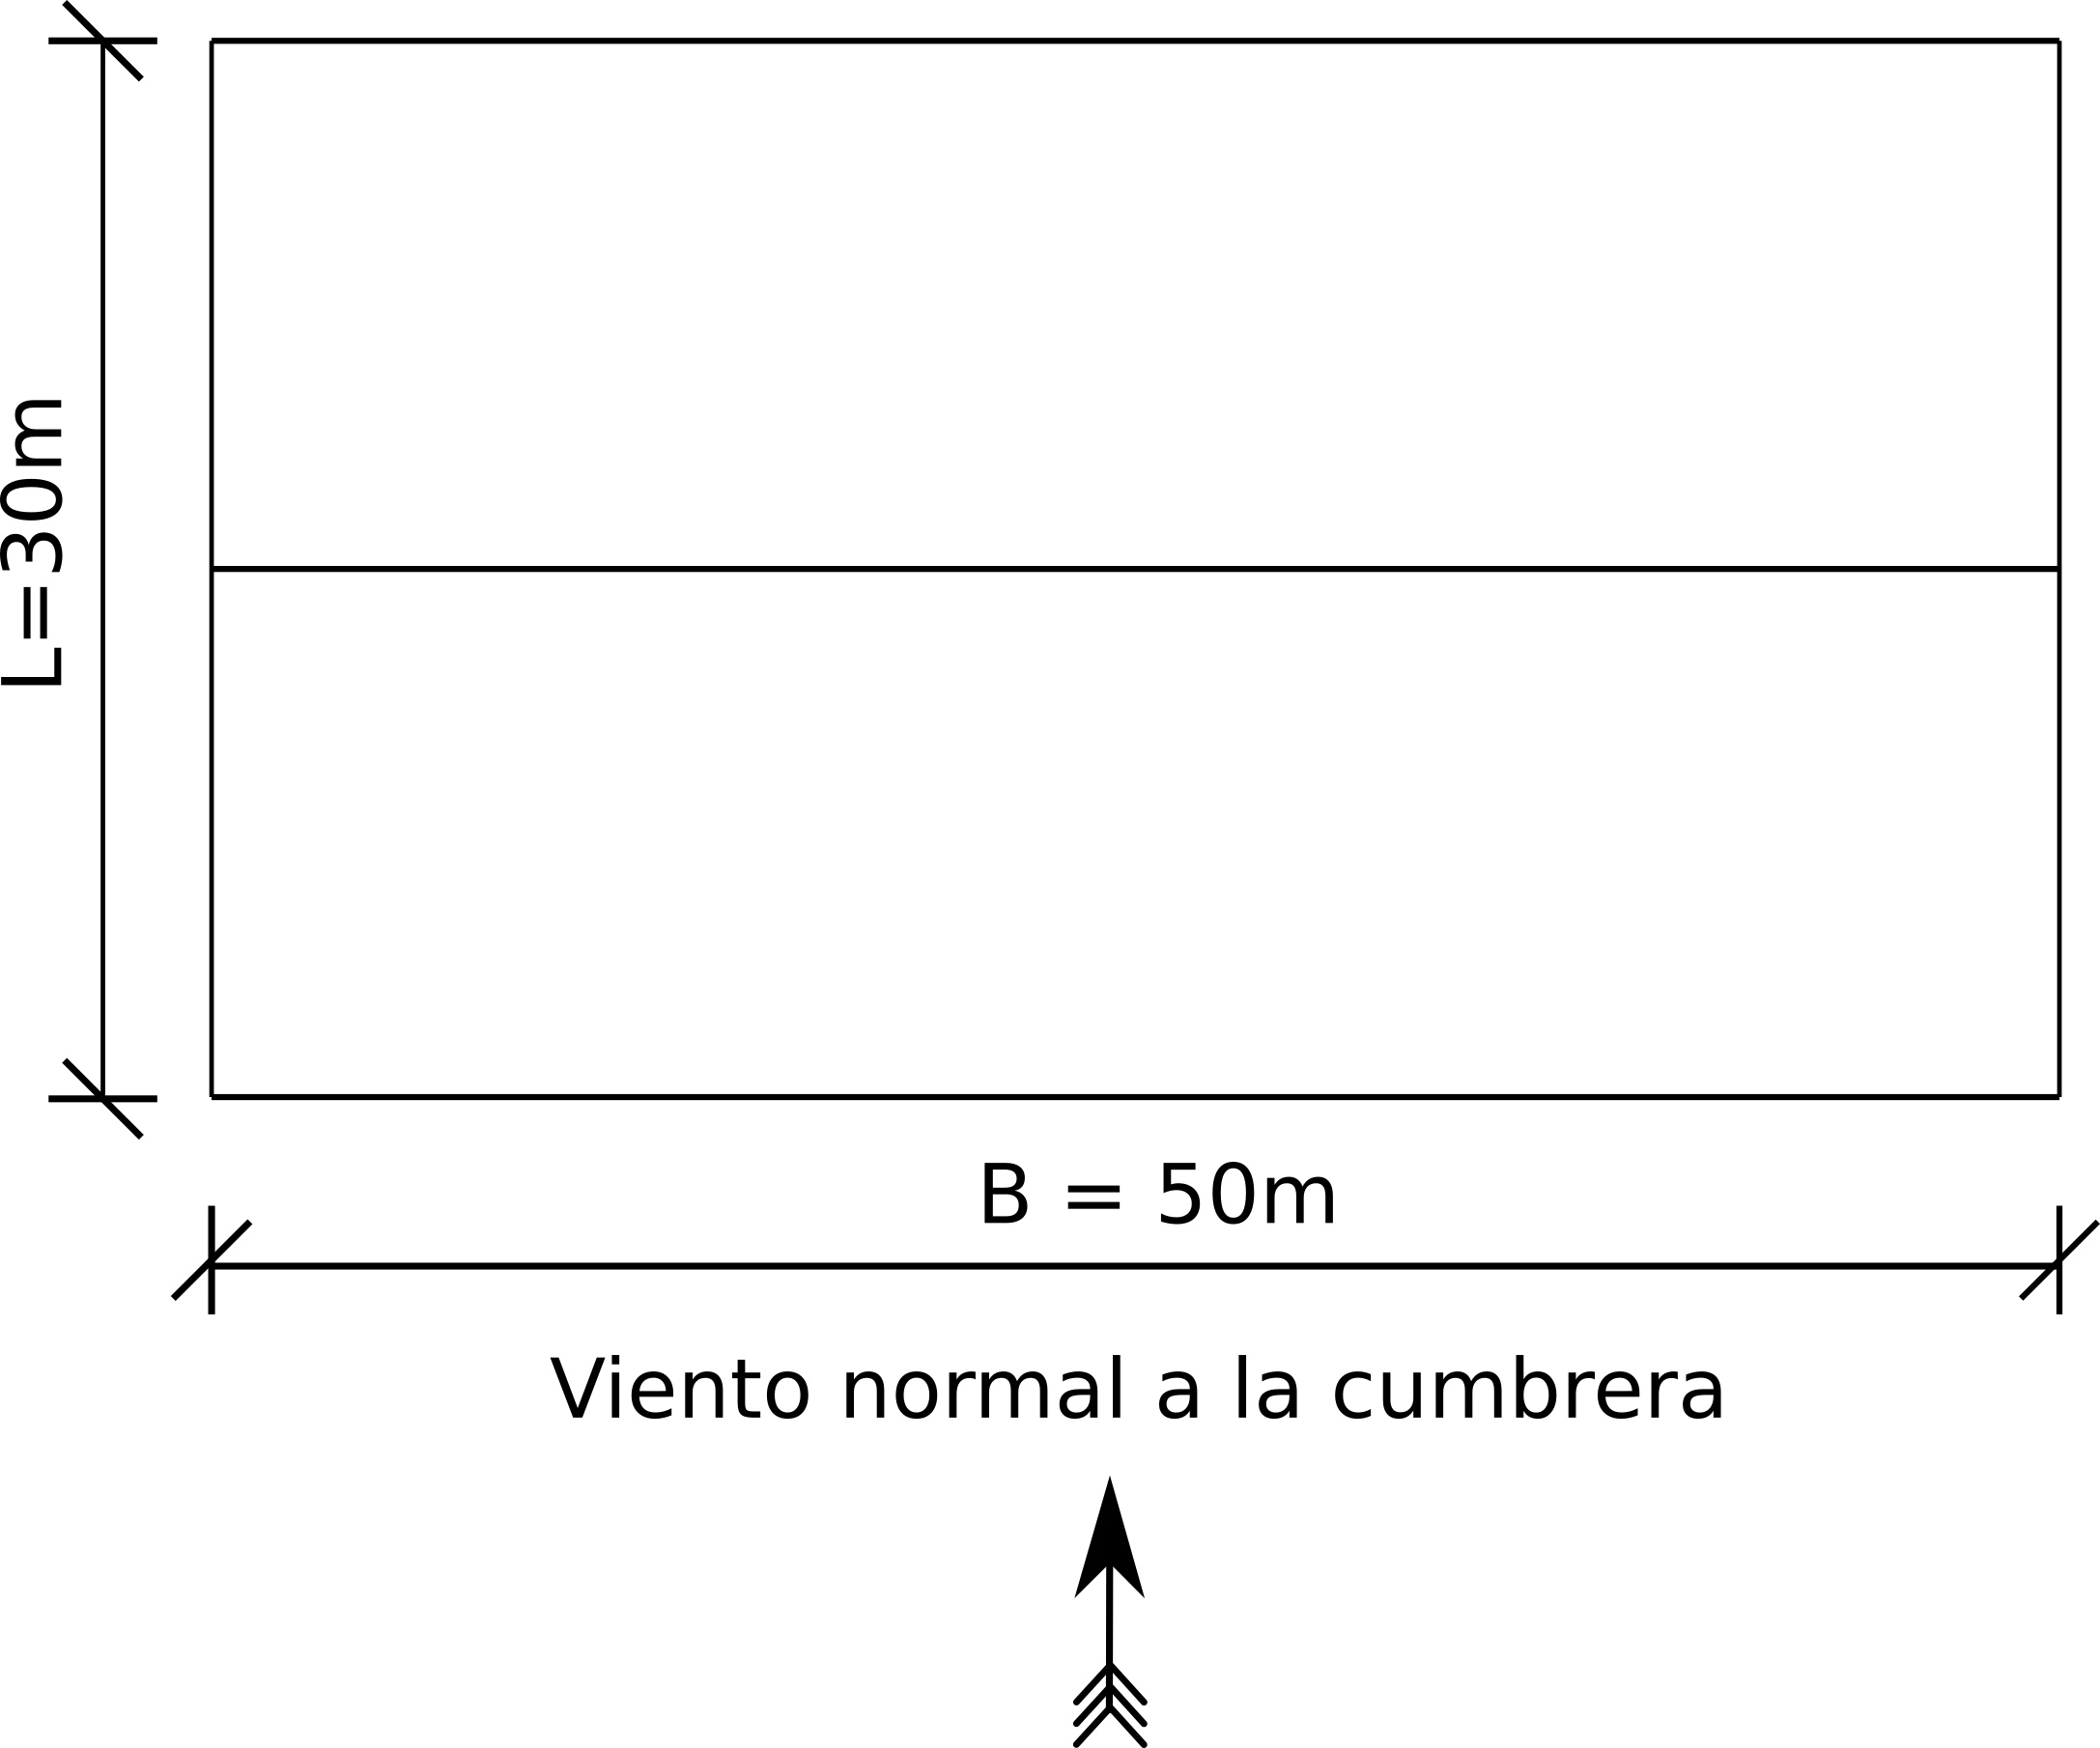
\includegraphics[scale = 0.7]{chapters/chapter_1/images/figura2.png}
\end{center}
\end{figure}

\[\left. \begin{array}{ll}
         \frac{L}{B}=\frac{30m}{50m}=0.6 & \\
         \frac{hmedia}{L}=\frac{9.43m}{30m}=0.314 & \end{array} \right\} \Rightarrow \text{Entrando en la Figura 3 e interpolando} \] 

\begin{table}[H]
  \begin{center}
    \begin{tabular}{l|c} % <-- Alignments: 1st column left, 2nd middle and 3rd right, with vertical lines in between
      Paredes & Cp \\
      \hline
      Barlovento & 0.8 \\
      Sotavento & -0.5 \\
      Laterales & -0.7 \\
    \end{tabular}
  \end{center}
\end{table}


\begin{table}[H]
  \begin{center}
    \begin{tabular}{l|c} % <-- Alignments: 1st column left, 2nd middle and 3rd right, with vertical lines in between
      Cubiertas $\theta =$ 18°& Cp \\
      \hline
      Barlovento & -0.41 \\
     			 & +0.09 \\ \hline
      Sotavento  & -0.56 \\
    \end{tabular}
  \end{center}
\end{table}

\item Viento $\parallel$ paralelo a la cumbrera
\begin{figure}[H]
\begin{center}
     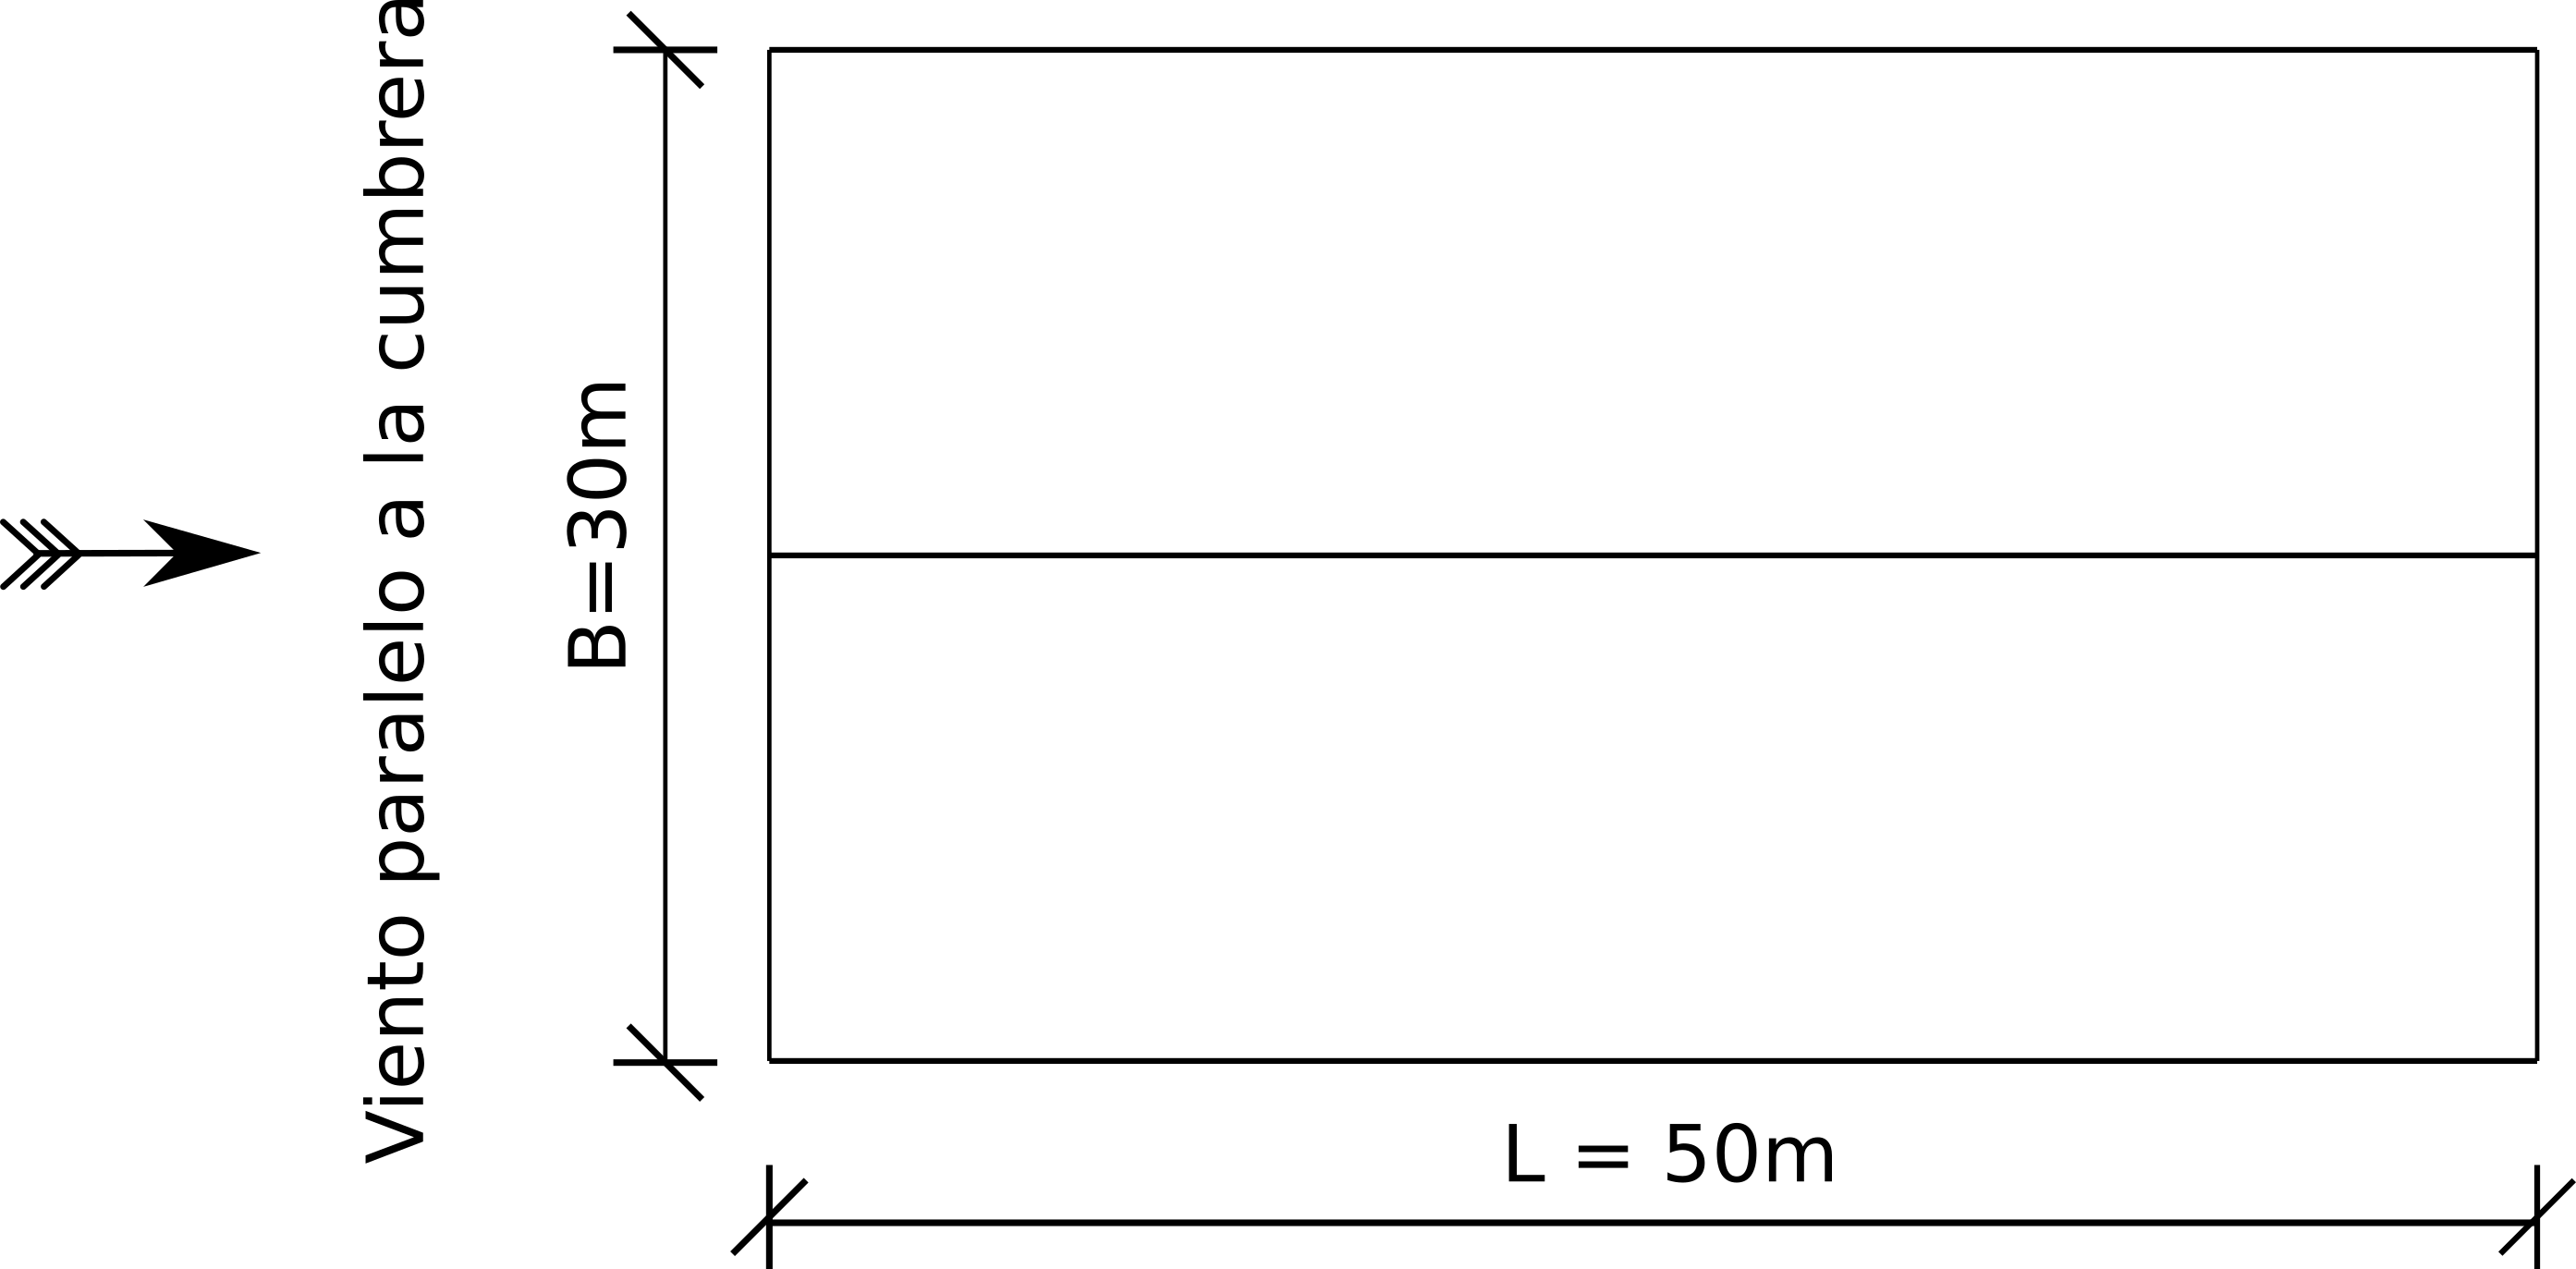
\includegraphics[scale = 0.7]{chapters/chapter_1/images/figura3.png}
\end{center}
\end{figure}

\[\left. \begin{array}{ll}
         \frac{L}{B}=\frac{50m}{30m}=1.66 & \\
         \frac{hmedia}{L}=\frac{9.43m}{50m}=0.18 & \end{array} \right\} \Rightarrow \text{Entrando en la Figura 3 e interpolando} \] 

\begin{table}[H]
  \begin{center}
    \begin{tabular}{l|c} % <-- Alignments: 1st column left, 2nd middle and 3rd right, with vertical lines in between
      Paredes & Cp \\
      \hline
      Barlovento & 0.8 \\
      Sotavento & -0.37 \\
      Laterales & -0.7 \\
    \end{tabular}
  \end{center}
\end{table}

\begin{table}[H]
  \begin{center}
    \begin{tabular}{l|c} % <-- Alignments: 1st column left, 2nd middle and 3rd right, with vertical lines in between
      Cubiertas & Cp \\ \hline
     0 a hmedia $\rightarrow$ 0 a 9.43m & -0.9 \\
     hmedia a $2 \cdot$ hmedia $\rightarrow$ 9.43m a 18.86m & -0.5 \\
     $> 2 \cdot$ hmedia  $\rightarrow$ > 18.86m & -0.3 \\
    \end{tabular}
  \end{center}
\end{table}
\end{itemize}

\begin{figure}[H]
\begin{center}
     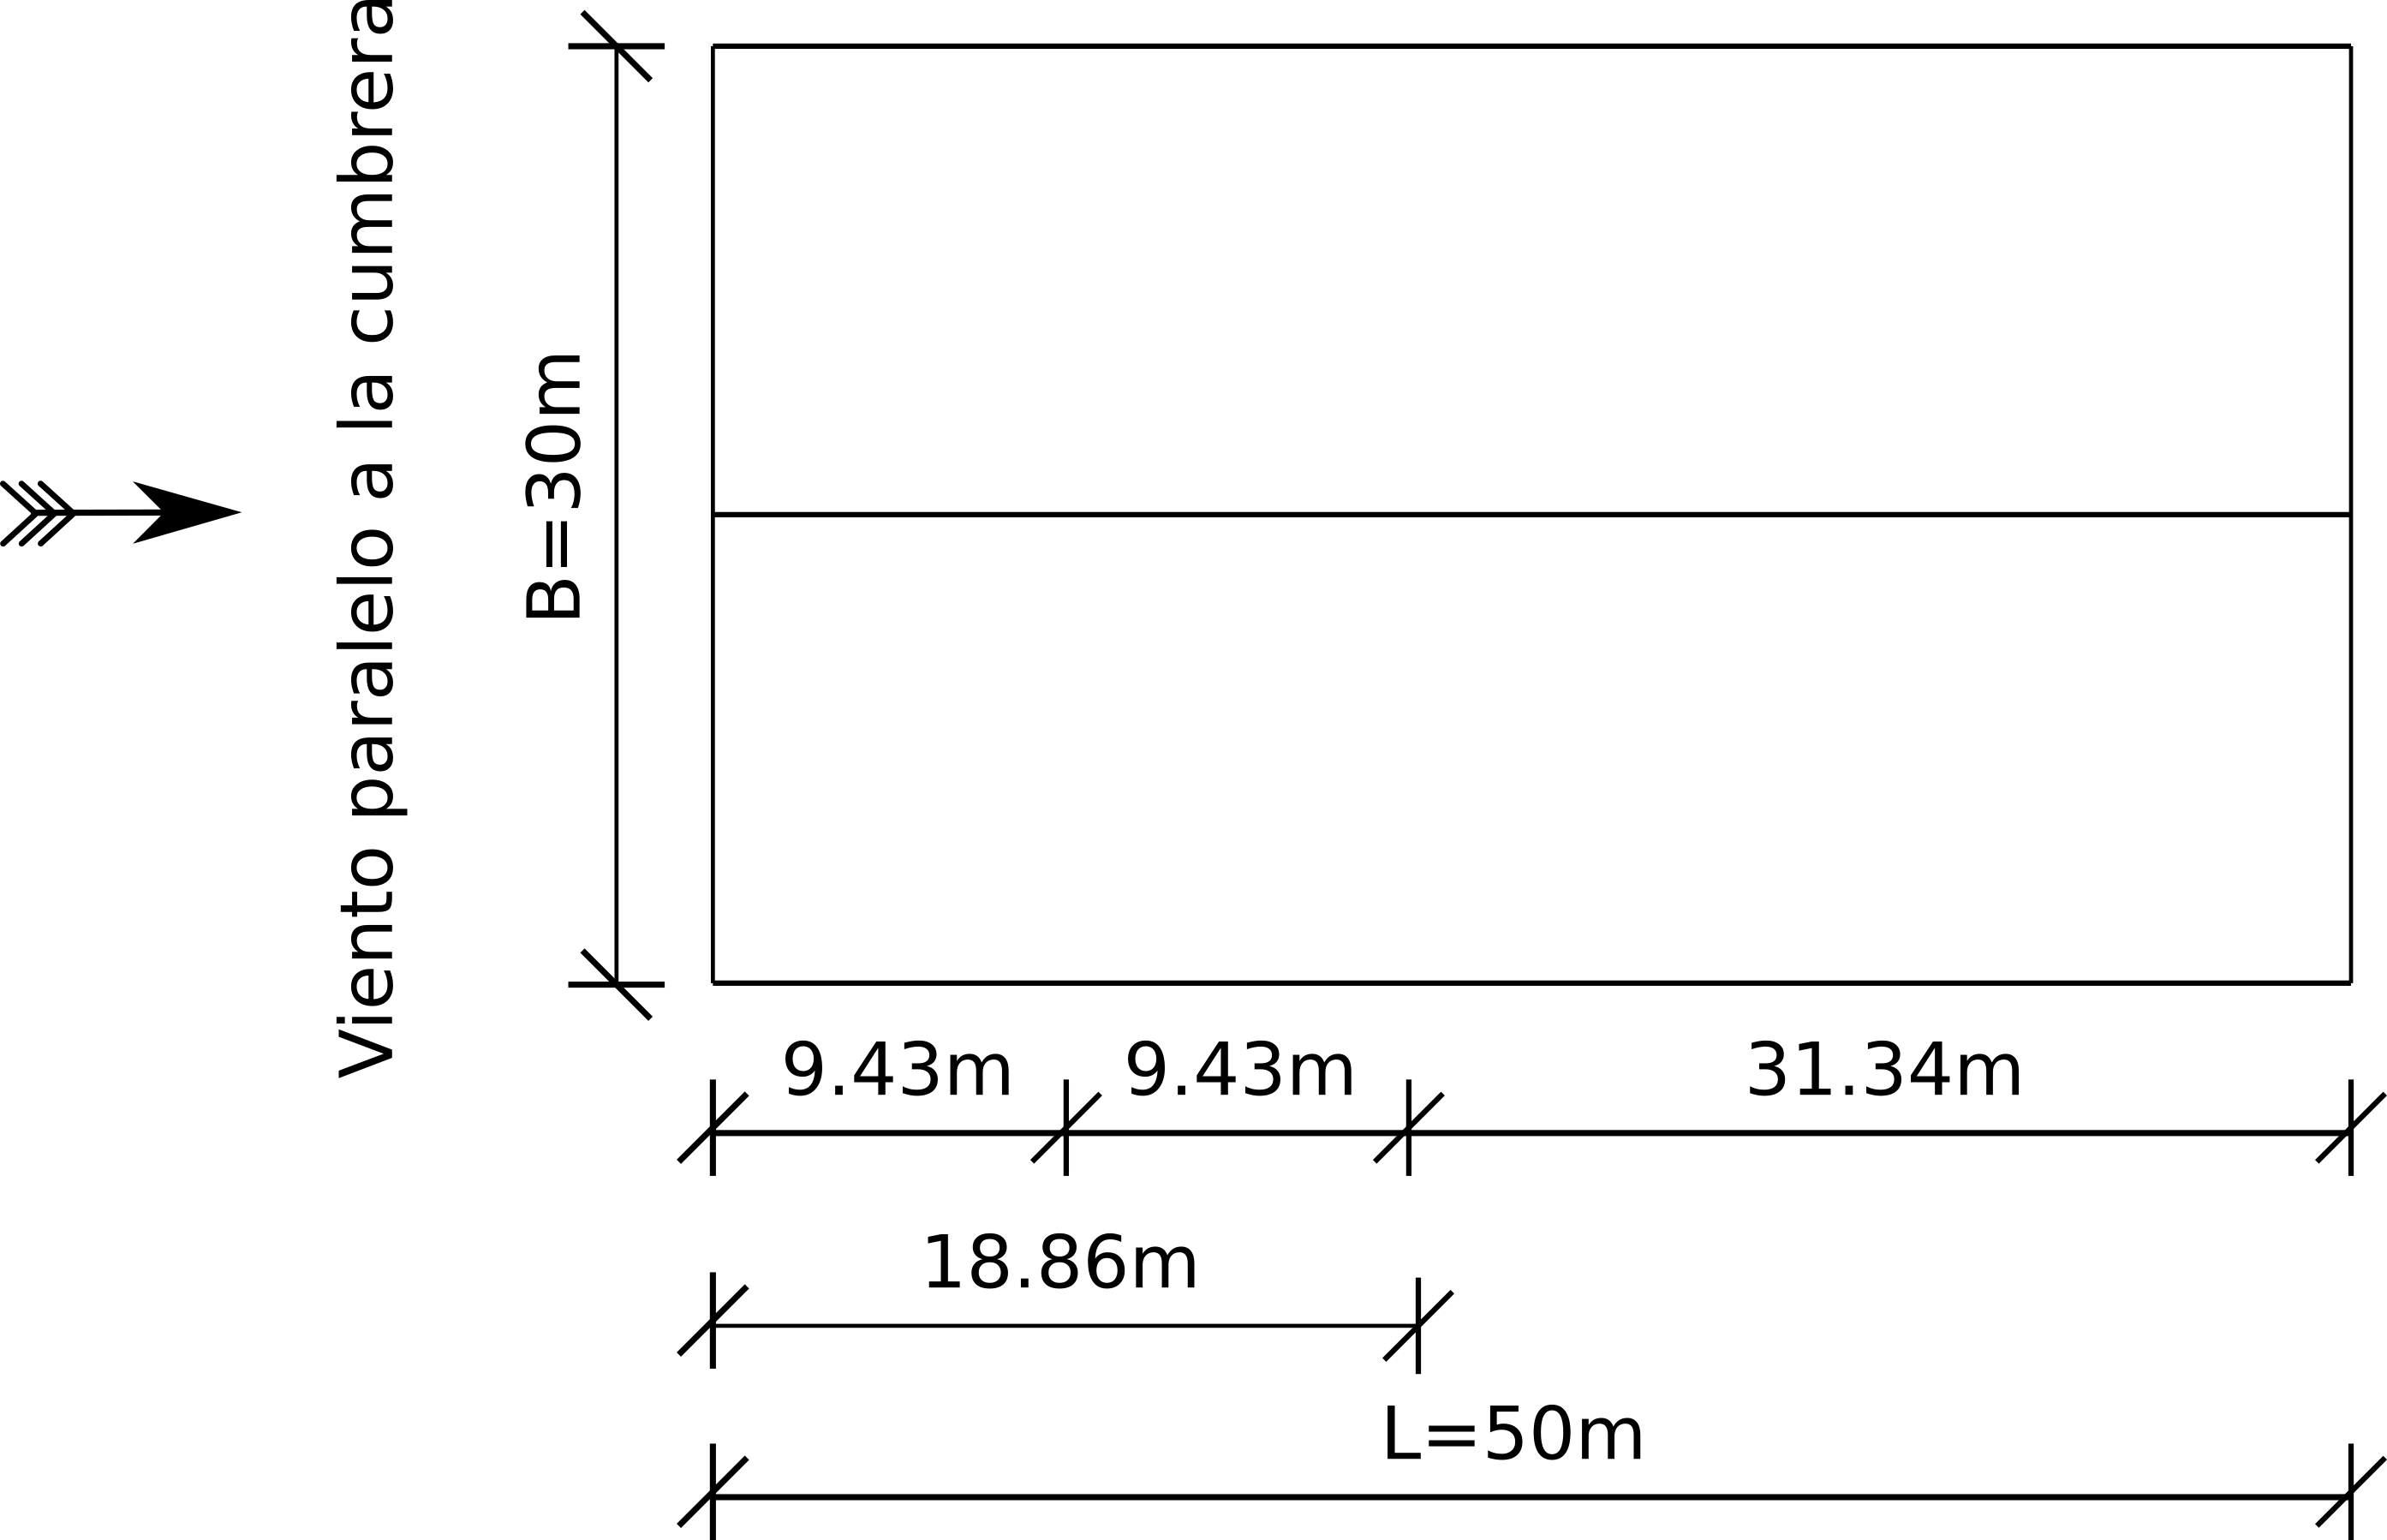
\includegraphics[scale = 0.7]{chapters/chapter_1/images/figura4.png}
\end{center}
\end{figure}

\item \underline{Presiones netas sobre el sistema principal resistente a la fuerza del viento}\\
\begin{itemize}
\item Viento $\perp$ normal a la cumbrera - Portón Cerrado

\begin{table}[H]
  \begin{center}
    \resizebox{\textwidth}{!}{\begin{tabular}{lccccccccc} \toprule
    Superficie & z & q & Cp & qGCp & qi & +GCpi & -GCpi & qGCp-qi(+GCpi) & qGCp-qi(-GCpi)\\ \midrule
	Pared a Barlovento 	&0-5		&2492,73	&0,8	&1695,06	&2753,87	&0,18	&-0,18	&1199,36	&2190,75 \\
						&6 			&2563,95	&0,8	&1743,49	&2753,87	&0,18	&-0,18	&1247.79	&2239,18 \\
						&7 			&2611,43	&0,8	&1775,77	&2753,87	&0,18	&-0,18	&1280,08	&2271,47\\  \midrule
Pared a Sotavento 		&Todas 		&2753,87	&-0,5	&-1170,39	&2753,87	&0,18	&-0,18	&-1666,09	&-674,70\\ \midrule
Paredes Laterales 		&Todas 		&2753,87	&-0,7	&-1638,55	&2753,87	&0,18	&-0,18	&-2134,25	&-1142,86\\ \midrule
Cubierta a barlovento   &			&2753,87	&-0,41	&-959,72	&2753,87	&0,18	&-0,18	&-1455,42	&-464,03 \\
				 	    &			&2753,87	&0,09	&210,67	    &2753,87	&0,18	&-0,18	&-285,03	&706,37 \\ \midrule
Cubierta a Sotavento    &			&2753,87	&-0,56	&-1310,84	&2753,87	&0,18	&-0,18	&-1806,54	&-815,15\\ \bottomrule
	\end{tabular}}
    \end{center}
\end{table}
\begin{align*}
&q_i \cdot GCpi = 2753.87\frac{N}{m^2} \cdot 0.18 = 495.70\frac{N}{m^2} \quad\text{Presión interna positiva} \\
&q_i \cdot -GCpi = 2753.87\frac{N}{m^2} \cdot -0.18 = -495.70\frac{N}{m^2} \quad\text{Presión interna negativa}
\end{align*}

\newpage
Presión interna positiva y cubierta a barlovento con coeficiente Cp=-0.41\\
\begin{figure}[H]
\begin{center}
     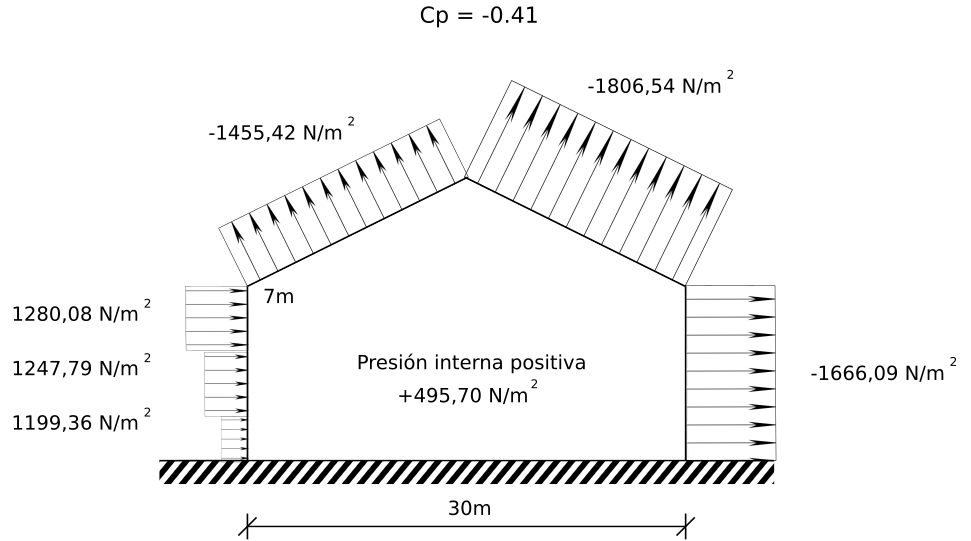
\includegraphics[scale = 0.4]{chapters/chapter_1/images/figura5.png}
\end{center}
\end{figure}

Presión interna negativa y cubierta a barlovento con coeficiente Cp=-0.41\\
\begin{figure}[H]
\begin{center}
     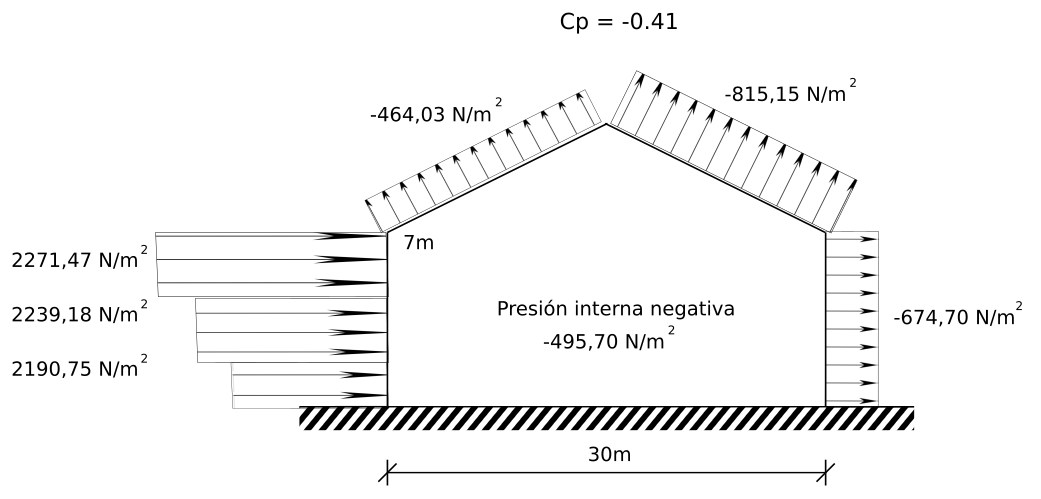
\includegraphics[scale = 0.4]{chapters/chapter_1/images/figura6.png}
\end{center}
\end{figure}

\newpage
Presión interna positiva y cubierta a barlovento con coeficiente Cp=0.09\\
\begin{figure}[H]
\begin{center}
     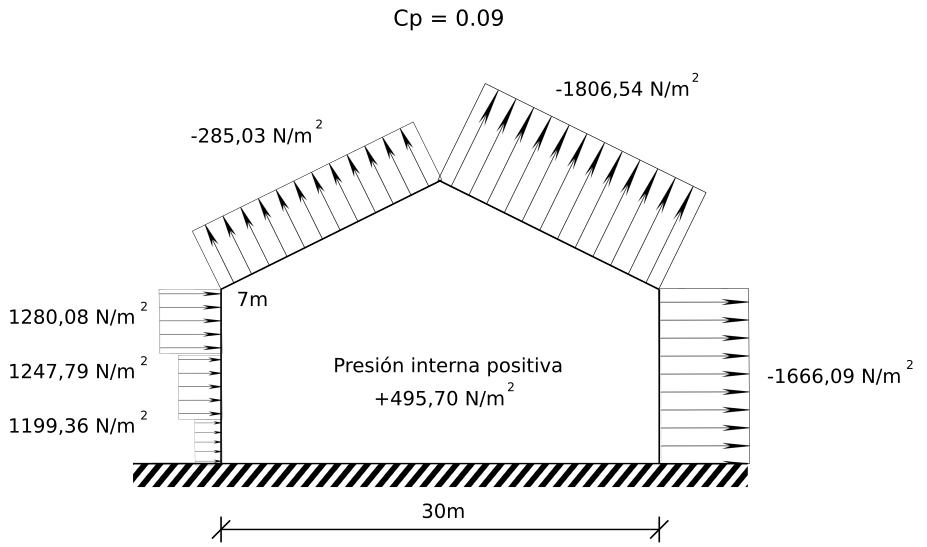
\includegraphics[scale = 0.4]{chapters/chapter_1/images/figura7.png}
\end{center}
\end{figure}

Presión interna negativa y cubierta a barlovento con coeficiente Cp=0.09\\
\begin{figure}[H]
\begin{center}
     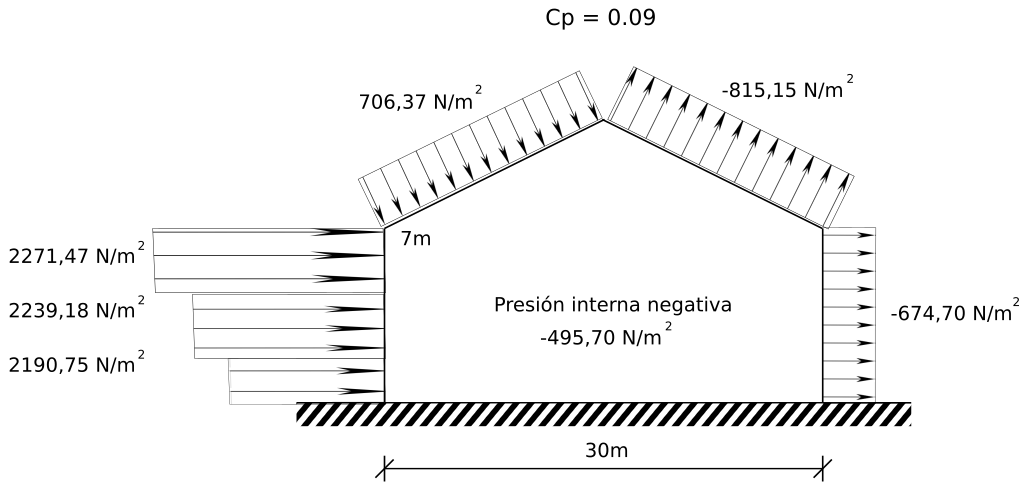
\includegraphics[scale = 0.4]{chapters/chapter_1/images/figura8.png}
\end{center}
\end{figure}

\newpage
\item Viento $\parallel$ paralelo a la cumbrera - Portón Abierto


\begin{table}[H]
  \begin{center}
    \resizebox{\textwidth}{!}{\begin{tabular}{lccccccccc} \toprule
    Superficie & z & q & Cp & qGCp & qi & +GCpi & -GCpi & qGCp-qi(+GCpi) & qGCp-qi(-GCpi)\\ \midrule

Pared a Barlovento 			&0-5		&2492,73	&0,8	&1695,06	&2753,87	&0,55	&-0,55	&180,43		&3209,68\\
		   					&6			&2563,95	&0,8	&1743,49	&2753,87	&0,55	&-0,55	&228,86		&3258,11\\
		   					&7			&2611,43	&0,8	&1775,77	&2753,87	&0,55	&-0,55	&261,14		&3290,40\\
	          				&9,43		&2753,87	&0,8	&1872,63	&2753,87	&0,55	&-0,55	&358,00		&3387,26\\
	          				&10			&2801,36	&0,8	&1904,92	&2753,87	&0,55	&-0,55	&390,30		&3419,55\\
	         				&11,87		&2872,58	&0,8	&1953,35	&2753,87	&0,55	&-0,55	&438,73		&3467,98\\ \midrule
Pared a Sotavento 			&Todas		&2753,87	&-0,37	&-866,09	&2753,87	&0,55	&-0,55	&-2380,72	&648,54\\ \midrule
Paredes Laterales 			&Todas		&2753,87	&-0,7	&-1638,55	&2753,87	&0,55	&-0,55	&-3153,18	&-123,92\\ \midrule
Cubierta				&0 a hmedia		&2753,87	&-0,9	&-2106,71	&2753,87	&0,55	&-0,55	&-3621,34	&-592,08\\
					&hmedia a 2.hmedia	&2753,87	&-0,5	&-1170,39	&2753,87	&0,55	&-0,55	&-2685,02	&344,23\\
					&>2.hmedia			&2753,87	&-0,3	&-702,24	&2753,87	&0,55	&-0,55	&-2216,87	&812,39\\ \bottomrule
		\end{tabular}}
    \end{center}
\end{table}

\begin{align*}
&q_i \cdot GCpi = 2753.87\frac{N}{m^2} \cdot 0.55 = 1514.63\frac{N}{m^2} \quad\text{Presión interna positiva} \\
&q_i \cdot -GCpi = 2753.87\frac{N}{m^2} \cdot -0.55 = -1514.63\frac{N}{m^2} \quad\text{Presión interna negativa}
\end{align*}

Presión interna positiva.\\
\begin{figure}[H]
\begin{center}
     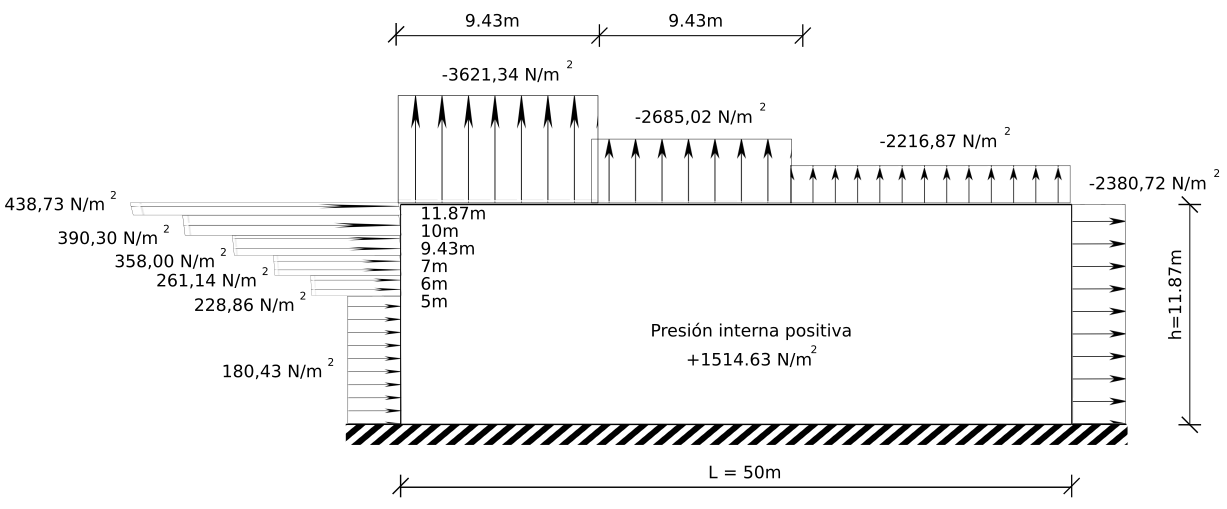
\includegraphics[scale = 0.4]{chapters/chapter_1/images/figura9.png}
\end{center}
\end{figure}

\begin{figure}[H]
\begin{center}
     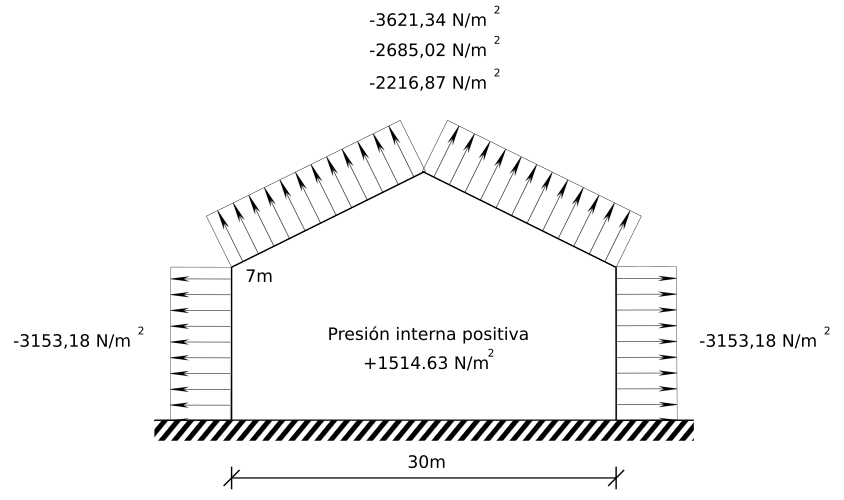
\includegraphics[scale = 0.5]{chapters/chapter_1/images/figura10.png}
\end{center}
\end{figure}

Presión interna negativa.\\
\begin{figure}[H]
\begin{center}
     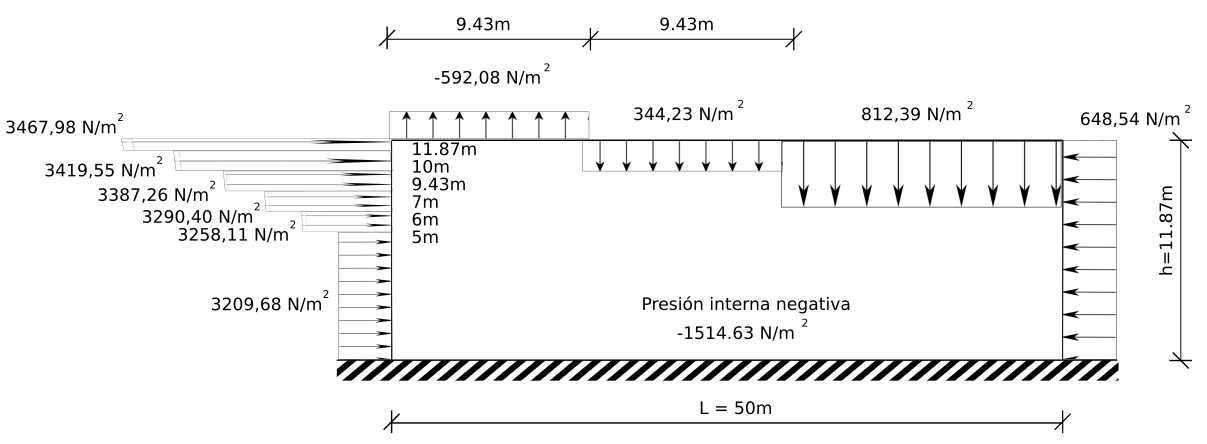
\includegraphics[scale = 0.4]{chapters/chapter_1/images/figura11.png}
\end{center}
\end{figure}

\begin{figure}[H]
\begin{center}
     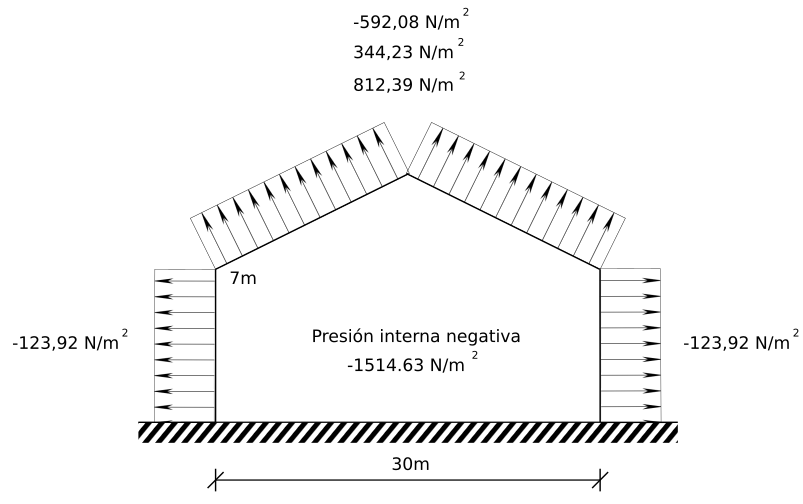
\includegraphics[scale = 0.5]{chapters/chapter_1/images/figura12.png}
\end{center}
\end{figure}

\item Viento $\parallel$ paralelo a la cumbrera - Portón Cerrado

\begin{table}[H]
  \begin{center}
    \resizebox{\textwidth}{!}{\begin{tabular}{lccccccccc} \toprule
    Superficie & z & q & Cp & qGCp & qi & +GCpi & -GCpi & qGCp-qi(+GCpi) & qGCp-qi(-GCpi)\\ \midrule

Pared a Barlovento 	&0-5				&2492,73	&0,8	&1695,06		&2753,87	&0,18	&-0,18	&1199,36	&2190,75\\
		   			&6					&2563,95	&0,8	&1743,49		&2753,87	&0,18	&-0,18	&1247,79	&2239,18\\
		   			&7					&2611,43	&0,8	&1775,77		&2753,87	&0,18	&-0,18	&1280,08	&2271,47\\
	          		&9,43				&2753,87	&0,8	&1872,63		&2753,87	&0,18	&-0,18	&1376,94	&2368,33\\
	          		&10					&2801,36	&0,8	&1904,92		&2753,87	&0,18	&-0,18	&1409,23	&2400,62\\
	         		&11,87				&2872,58	&0,8	&1953,35		&2753,87	&0,18	&-0,18	&1457,66	&2449,05\\  \midrule
Pared a sotavento 	&Todas				&2753,87	&-0,37	&-866,09		&2753,87	&0,18	&-0,18	&-1361,79	&-370,40\\  \midrule
Paredes Laterales 	&Todas				&2753,87	&-0,7	&-1638,55		&2753,87	&0,18	&-0,18	&-2134,25	&-1142,86\\  \midrule
Cubierta	  		&0 a hmedia			&2753,87	&-0,9	&-2106,71		&2753,87	&0,18	&-0,18	&-2602,41	&-1611,01\\
					&hmedia a 2.hmedia	&2753,87	&-0,5	&-1170,39		&2753,87	&0,18	&-0,18	&-1666,09	&-674,70\\
					&>2.hmedia			&2753,87	&-0,3	&-702,24		&2753,87	&0,18	&-0,18	&-1197,93	&-206,54\\ \bottomrule
		\end{tabular}}
    \end{center}
\end{table}

\begin{align*}
&q_i \cdot GCpi = 2753.87\frac{N}{m^2} \cdot 0.18 = 495.70\frac{N}{m^2} \quad\text{Presión interna positiva} \\
&q_i \cdot -GCpi = 2753.87\frac{N}{m^2} \cdot -0.18 = -495.70\frac{N}{m^2} \quad\text{Presión interna negativa}
\end{align*}

\newpage
Presión interna positiva.\\
\begin{figure}[H]
\begin{center}
     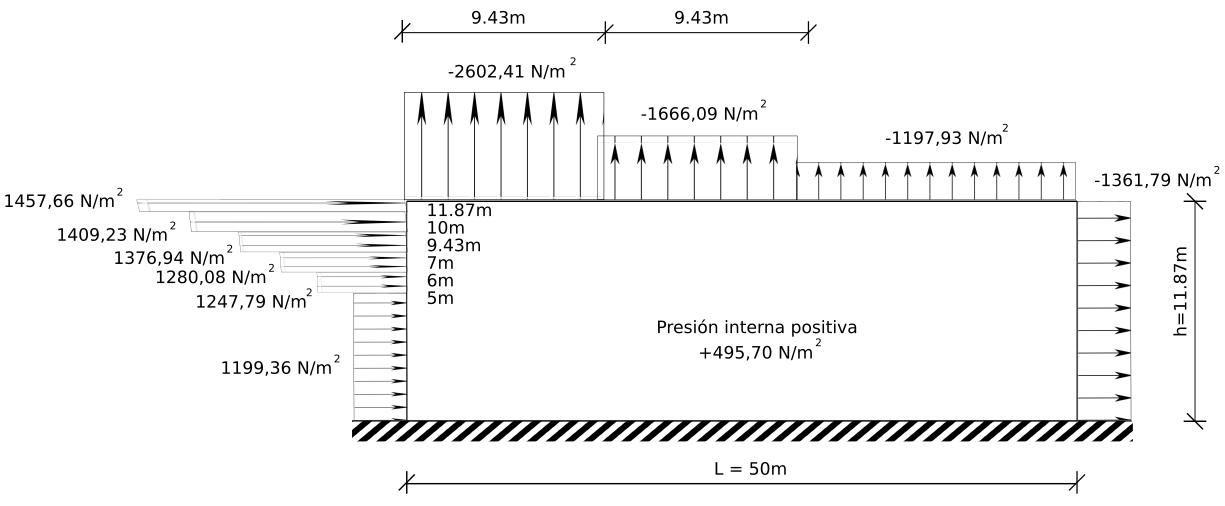
\includegraphics[scale = 0.4]{chapters/chapter_1/images/figura13.png}
\end{center}
\end{figure}

\begin{figure}[H]
\begin{center}
     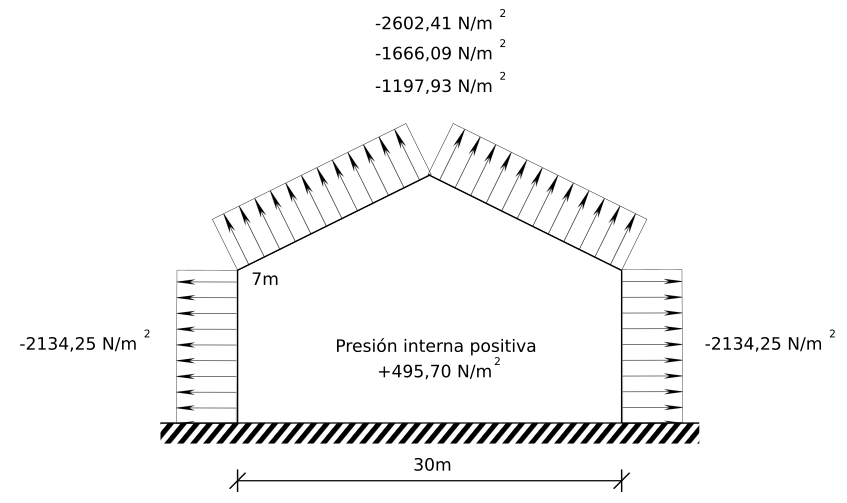
\includegraphics[scale = 0.5]{chapters/chapter_1/images/figura14.png}
\end{center}
\end{figure}

\newpage
Presión interna negativa.\\
\begin{figure}[H]
\begin{center}
     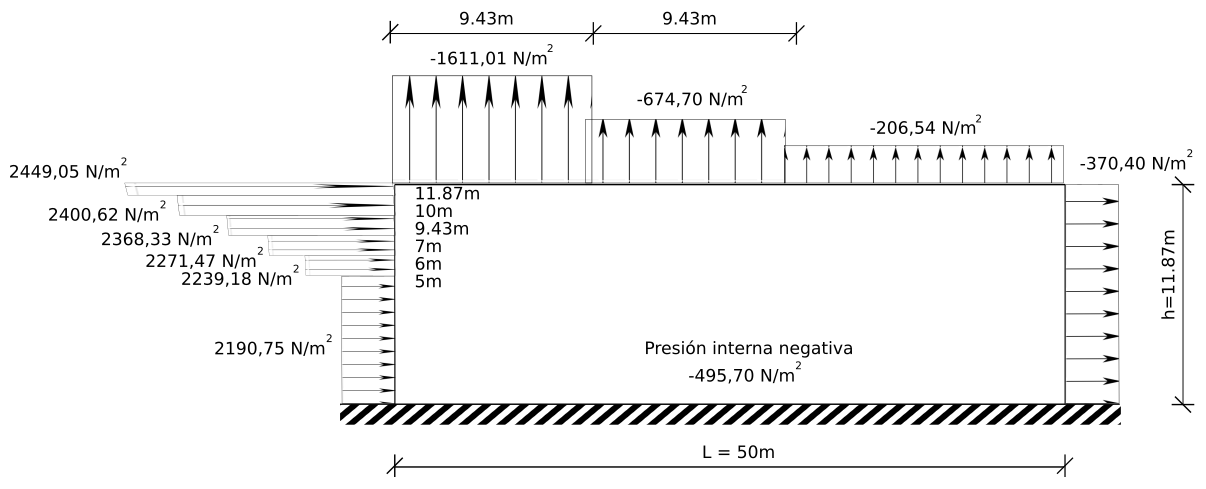
\includegraphics[scale = 0.4]{chapters/chapter_1/images/figura15.png}
\end{center}
\end{figure}

\begin{figure}[H]
\begin{center}
     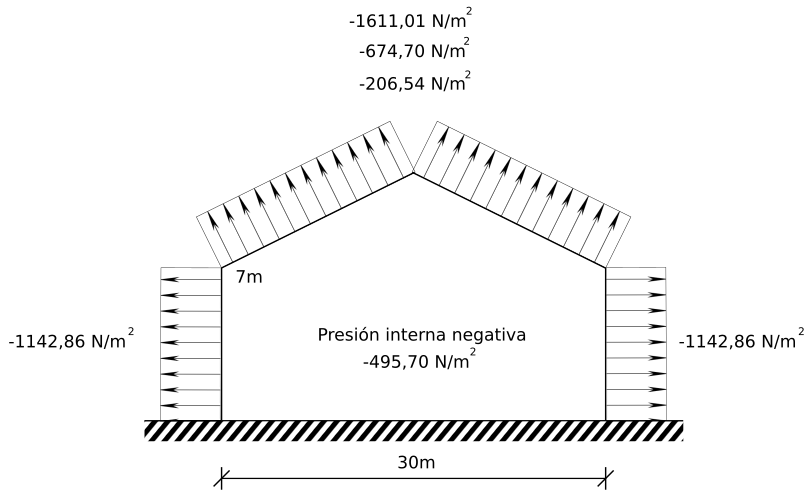
\includegraphics[scale = 0.5]{chapters/chapter_1/images/figura16.png}
\end{center}
\end{figure}

\end{itemize}
\end{enumerate}

